\documentclass{beamer}
\usepackage{workshop}

\begin{document}

\title{Introduction to Python 0 -- How to run Python}
\date{May 2015}
\author{Chang Y. Chung}
\institute{Office of Population Research}

% -----------------------------------------------
{\setbeamertemplate{footline}{}
\begin{frame}[noframenumbering]
%{\color{red}D R A F T}
\titlepage
\end{frame}}

% -----------------------------------------------
\begin{frame}[fragile]
\frametitle{Schedule}
\begin{table}[h]
\scalebox{0.7}{
    \begin{tabular}{@{}rcrp{0.7\linewidth}l@{}}
    \toprule
    from &   & to & topic & note \\
    \midrule
    9:30am & - & 10:30am & How to run Python; Comments; Variables;
        Integers and Floating point numbers; Strings; None; 
        Operators  & \\
    10:30am & - & 11:00am & Break & \\
    11:00am & - & noon & Flow Control and Compound statements;
        File I/O; Defining and Calling a Function; Local and
        Global Variables; Importing a module & \\
    noon & - & 1:30pm & Lunch break & \#242 \\
    1:30pm & - & 2:30pm & List; Dictionary; Data Structure & \\
    2:30pm & - & 3:00pm & Break and Optional Evaluation & \\
    3:00pm & - & 4:00pm & Tuples; Class; Exception Handling;
        Regular Expression & \\
    \bottomrule
    \end{tabular}
}
\end{table}
\end{frame}

% -----------------------------------------------
\begin{frame}[fragile]
\frametitle{Running Python Read-Eval-Print Loop 1}
\begin{itemize}
\item For those who are using UNIX-like systems,
      including Apple Mac, Nobel, or Adroit.
\item On Mac, open the terminal window.
\begin{figure}[h]
    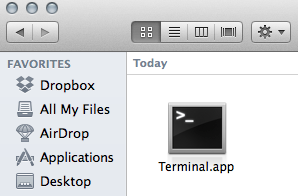
\includegraphics[width=4cm]{macterm.png}
\end{figure}
\end{itemize}
\end{frame}

% -----------------------------------------------
\begin{frame}[fragile]
\frametitle{Running Python Read-Eval-Print Loop 2}
\begin{itemize}
\item Skip this step, if you are running locally installed Python.
Continue, if you are to run Python on Nobel or Adroit.
\item Register for an account at:
\url{http://www.princeton.edu/researchcomputing/computational-hardware/}
\item Secure Shell (ssh) into Nobel (or Adroit).
\begin{figure}[h]
    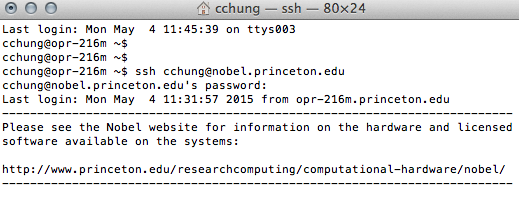
\includegraphics[width=9cm]{nobelssh.png}
\end{figure}
\end{itemize}
\end{frame}

% -----------------------------------------------
\begin{frame}[fragile]
\frametitle{Running Python Read-Eval-Print Loop 3}
\begin{itemize}
\item Run Python REPL at the shell prompt.
\begin{figure}[h]
    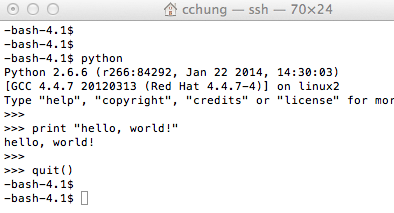
\includegraphics[width=8cm]{nobelrepl.png}
\end{figure}
\end{itemize}
\end{frame}
% -----------------------------------------------

\begin{frame}[fragile]
\frametitle{Running a Python Script File (.py)}
\begin{itemize}
\item Create a python script file using a text editor
    (nano, vim, emacs, ...).
\item Type "python" followed by the script file name 
    at the shell prompt.
\begin{figure}[h]
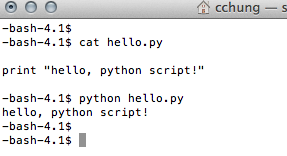
\includegraphics[width=7cm]{nobelscript.png}
\end{figure}
\end{itemize}
\end{frame}

% -----------------------------------------------
\begin{frame}[fragile]
\frametitle{Running a Local Python REPL on Windows 1}
\begin{itemize}
\item (MS Windows before 8) Open a cmd window.
\begin{figure}[h]
    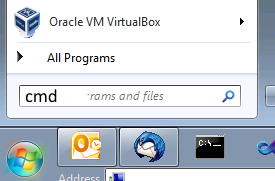
\includegraphics[width=5cm]{wincmd.png}
\end{figure}
\item (Ms Windows 8 and 8.1) Swipe up to show the Apps
     screen. Swipe or scroll to the right and click
     on the Command Prompt under the Windows System
     section.
\end{itemize}
\end{frame}

% -----------------------------------------------
\begin{frame}[fragile]
\frametitle{Running a Local Python REPL on Windows 2}
\begin{itemize}
\item Start Python REPL.
\begin{figure}[h]
    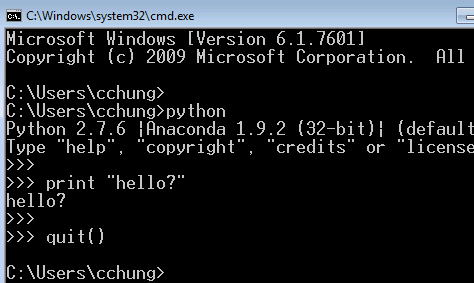
\includegraphics[width=7cm]{wincmdrepl.png}
\end{figure}
\end{itemize}
\end{frame}

% -----------------------------------------------
\begin{frame}[fragile]
\frametitle{Running a Python Script File (.py) on Windows}
\begin{itemize}
\item Create a python script file using a text editor
    (notepad, nano, vim, emacs, ...).
\item Execute python command with the script file name 
    at the shell prompt.
\begin{figure}[h]
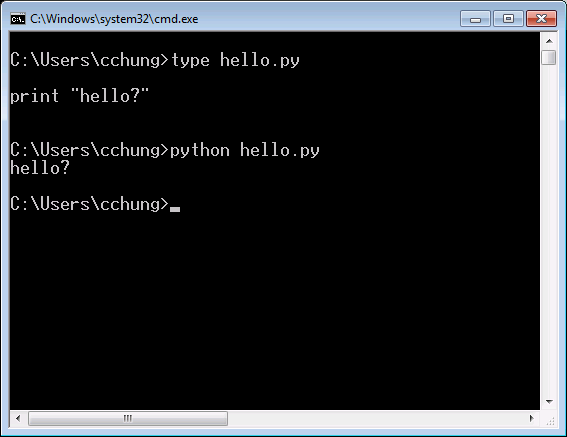
\includegraphics[width=7cm]{wincmdscript.png}
\end{figure}
\end{itemize}
\end{frame}

% -----------------------------------------------
\begin{frame}[fragile]
\frametitle{Starting IPython Notebook 1}
\begin{itemize}
\item For those who are using Apple Mac.
\item Open the terminal window.
\begin{figure}[h]
  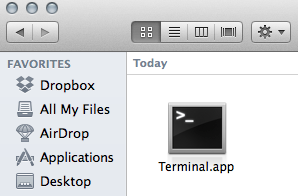
\includegraphics[width=4cm]{macterm.png}
\end{figure}
\end{itemize}
\end{frame}

% -----------------------------------------------
\begin{frame}[fragile]
\frametitle{Starting IPython Notebook 2}
\begin{itemize}
\item (Optional) Change directory to the desired sub-directory.
\item Execute "ipython notebook" command. The default browser
    should open up showing the current working directory. 
\begin{figure}[h]
  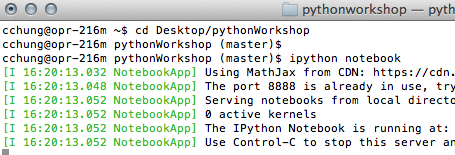
\includegraphics[width=8cm]{startjupyter.png}
\end{figure}
\end{itemize}
\end{frame}

% -----------------------------------------------
\begin{frame}[fragile]
\frametitle{Starting IPython Notebook 3}
\begin{itemize}
\item Either open an existing ipython notebook (.ipynb)
    or create a new one (click on Python 2 under New $>$ Notebooks)
\begin{figure}[h]
  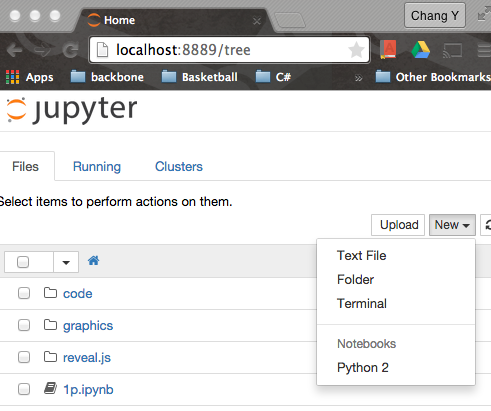
\includegraphics[width=7cm]{jupytertree.png}
\end{figure}
\end{itemize}
\end{frame}

% -----------------------------------------------
\begin{frame}[fragile]
\frametitle{Quiz}
\begin{itemize}
\item Print out a "HELLO" in your environment.
\item Print out "HELLO" 20 times in your environment.
\item Print out "HELLO" \emph{vertically}, that is, the printed
output should look like below (line numbers are not required).
\begin{lstlisting}
H
E
L
L
O
\end{lstlisting} 
\end{itemize}
\end{frame}

% -----------------------------------------------
% \begin{frame}%[allowframebreaks]
%   \frametitle{References}
%   \bibliographystyle{acm}
%   \scriptsize
%   \bibliography{references}
% \end{frame}
 
\end{document}
